\chapter{Kiemelt modulok a frontendben}

A WaccApp frontendjének kiemelt moduljai azokhoz a felhasználói folyamatokhoz kapcsolódnak, amelyek a rendszer gyakorlati értékét adják. A 7. fejezet bemutatta, hogy a frontend több, feladat szerint elkülönített HTML-nézetből épül fel. Ebben a fejezetben már nem a szerkezet önmagában, hanem az egyes modulok tényleges működése kerül előtérbe. A cél annak bemutatása, hogy az üzenetküldés, a beszélgetésmegjelenítés, a kérdőívszerkesztés, a szűrés, a médiafájl-kezelés és az időzített küldés hogyan jelenik meg konkrét frontendfolyamatként. 

A fejezet ezért nem általános frontendelveket ismétel meg, hanem a WaccApp saját nézeteit és azok szerepét elemzi. Az \path{index.html} a műveletindítás központi felületeként jelenik meg, a \path{messages.html} és a \path{sent-messages.html} az üzenetek listaalapú visszakövetését támogatja, a \path{conv.html} a kontaktalapú beszélgetésértelmezés nézete, a \path{questionnaire.html} és a sablonkezelő oldalak a kérdőíves folyamatok szerkesztését teszik lehetővé, a \path{filter.html} pedig az adatok célzott visszakeresését és alapvető értelmezését biztosítja. A médiafájlokhoz és időzített küldésekhez kapcsolódó működés ezekhez a fő nézetekhez illeszkedik, és a kommunikációs folyamatot bővíti ki. 

\section{Üzenetküldés és beszélgetésnézet}

Az üzenetküldési modul a WaccApp egyik legfontosabb része, mert ezen keresztül indulnak azok a kommunikációs műveletek, amelyekre a rendszer többi funkciója is ráépül. A modul nem egyetlen oldalból áll, hanem több, egymást kiegészítő nézet együttműködéséből. Az \path{index.html} a műveletindítás helye, a \path{messages.html} és a \path{sent-messages.html} az üzenetek listaalapú áttekintését teszi lehetővé, míg a \path{conv.html} egy adott kontakthoz kapcsolódó beszélgetést jelenít meg részletesebb, chat-szerű formában. 

Az \path{index.html} feladata az, hogy a felhasználó egy helyről tudja elindítani az alapvető küldési folyamatokat. Ezen a felületen külön kezelhető az egyszerű szöveges üzenet, a sablonos üzenet, a kérdőívindítás, a médiafájl küldése és az időzített küldés. A frontend szempontjából ennek az a jelentősége, hogy az oldalnak nem egyetlen merev űrlapot kell megjelenítenie, hanem a kiválasztott művelethez igazodó adatbeviteli helyzetet. Egyszerű szöveges üzenetnél a címzett és az üzenetszöveg a meghatározó, sablonos küldésnél viszont a sablonnév, a nyelvi beállítás és a paraméterek is szükségessé válnak. A felület így nem terheli a felhasználót minden esetben az összes lehetőséggel, hanem a választott küldési módhoz igazítja a szükséges mezőket.

\begin{figure}[H]
\centering
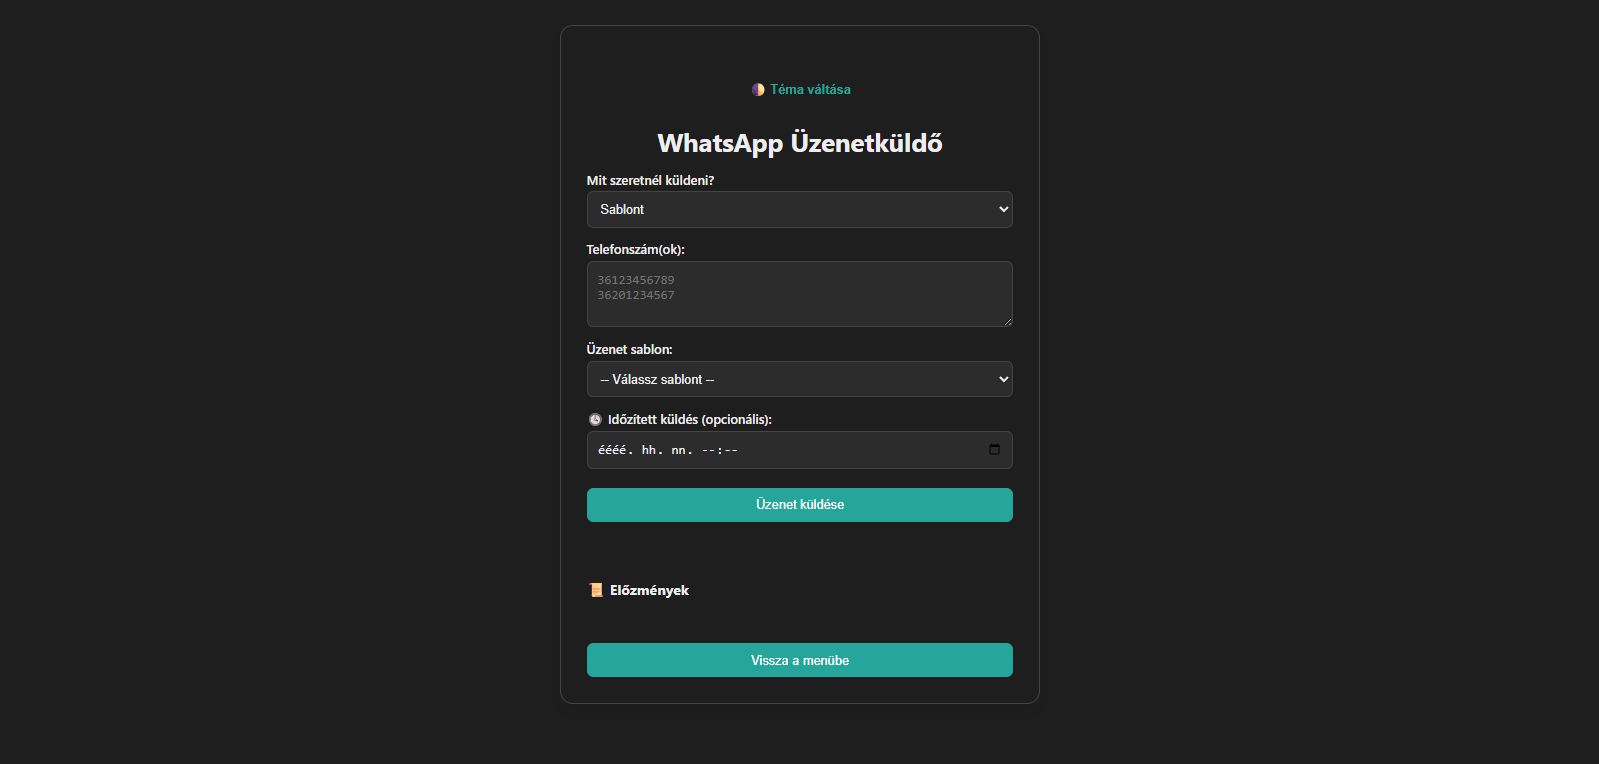
\includegraphics[width=0.95\textwidth]{images/index-html.png}
\caption{Az index.html központi üzenetküldő felülete}
\label{fig:index-html}
\end{figure}

A képernyőképen látható felület azt szemlélteti, hogy a WaccApp-ban a küldési műveletek nem különálló, egymástól elszakított funkcióként jelennek meg, hanem egy közös indítófelülethez kapcsolódnak. Ez a megoldás a felhasználó számára egyszerűbb belépési pontot ad, miközben a háttérben eltérő adatcsomagok és API-hívások indulhatnak el. A nézet ezért jól mutatja a dolgozat egyik alapvető frontendtervezési döntését: a technikai WhatsApp API-műveletek felhasználói munkafolyamattá alakítását.

A küldési folyamat frontendoldali működését jól szemlélteti az \path{index.html} egyik egyszerűsített részlete. A kódrészlet azt a részt mutatja be, ahol a felület a telefonszámokat feldolgozza, ellenőrzi, majd a kiválasztott küldési mód alapján vagy fájlküldést, vagy szöveges üzenetküldést indít.

\begin{CodeBlock}
const phonesRaw = document.getElementById('phone').value.trim();
const phones = phonesRaw
  .split(/\s|,|;/)
  .map(p => p.trim())
  .filter(p => p.length > 0);

const invalidPhones = phones.filter(p => !/^36\d{8,}$/.test(p));

if (invalidPhones.length > 0) {
  statusDiv.textContent =
    `Hibás formátumú szám(ok): ${invalidPhones.join(', ')}.`;
  statusDiv.style.color = 'crimson';
  return;
}

if (phones.length === 0) {
  statusDiv.textContent = 'Kérlek, adj meg legalább egy telefonszámot.';
  statusDiv.style.color = 'crimson';
  return;
}

statusDiv.textContent = 'Üzenet(ek) küldése...';

if (fileInput.files.length > 0) {
  phones.forEach(phone => {
    const formData = new FormData();
    formData.append('phone', phone);
    formData.append('message', fullMessage);
    formData.append('file', fileInput.files[0]);

    fetch('/send-file-message', {
      method: 'POST',
      body: formData
    })
      .then(r => r.json())
      .then(d => handleResponse(d, phone, fullMessage));
  });
} else {
  phones.forEach(phone => {
    const payload = { phone, message: fullMessage };

    fetch('/send-message', {
      method: 'POST',
      headers: { 'Content-Type': 'application/json' },
      body: JSON.stringify(payload)
    })
      .then(r => r.json())
      .then(d => handleResponse(d, phone, fullMessage));
  });
}
\end{CodeBlock}

A részlet alapján látható, hogy a frontend nem közvetlenül továbbítja a beírt adatokat, hanem először értelmezhető szerkezetbe rendezi őket. A telefonszámok többféle elválasztással is megadhatók, a kliensoldal ezekből külön címzettlistát állít elő, majd kiszűri a hibás formátumú elemeket. A validáció után a rendszer ugyanazon felületi folyamatból két eltérő küldési utat tud indítani: fájl esetén FormData alapú kérést küld a /send-file-message végpontra, egyszerű szöveges üzenet esetén pedig JSON-adatot továbbít a /send-message végpontra. Ez a megoldás jól mutatja a WaccApp frontendjének egyik lényeges szerepét: a felhasználói adatbevitelből a háttérrendszer számára feldolgozható kérést készít.

A küldési folyamatban a frontend elsődleges szerepe az, hogy a felhasználói szándékot a háttérrendszer számára feldolgozható adattá alakítsa. Ez azt jelenti, hogy a felület begyűjti a címzettet, a tartalmat, a sablonhoz tartozó paramétereket vagy a csatolt fájlt, majd a megfelelő végpont felé továbbítja a kérést. A felhasználó ebből nem az API-hívás technikai részleteit érzékeli, hanem azt, hogy a rendszer megköveteli a szükséges adatokat, jelzi a hiányzó mezőket, majd visszajelzést ad a művelet eredményéről. Ez különösen fontos, mert egy WhatsApp Business API-ra épülő rendszerben a hibás adatbevitel nemcsak lokális felületi hiba, hanem sikertelen küldési folyamat is lehet. [R13], [R14] 

A \path{messages.html} és a \path{sent-messages.html} a kommunikáció visszakövetését listaalapú formában támogatja. A beérkező és elküldött üzenetek külön nézetben történő kezelése azért hasznos, mert a felhasználó eltérő kérdésekre keres választ a két esetben. A beérkező üzeneteknél az a fontos, hogy milyen válaszok érkeztek a címzettektől, az elküldött tételeknél pedig az, hogy a rendszer milyen tartalmakat, mikor és milyen típusban továbbított. Ez a két nézet gyors ellenőrzésre alkalmas, de önmagában még nem mindig adja vissza egy teljes kommunikációs folyamat összefüggéseit. 

Ezt a hiányt a \path{conv.html} oldja fel, amely nem egyszerű adatlistaként, hanem beszélgetésfolyamként jeleníti meg a korábbi interakciókat. A nézet kontaktalapú logikája azért fontos, mert a felhasználó sokszor nem egy önálló üzenetet szeretne értelmezni, hanem azt, hogy egy adott személlyel vagy telefonszámmal milyen kommunikáció zajlott le. A bejövő és kimenő üzenetek elkülönítése, az időrendi megjelenítés és a chat-szerű forma a rendszer használatát közelebb viszi ahhoz a mintához, amelyet a felhasználók a hétköznapi üzenetküldő alkalmazásokból már ismernek. A WaccApp esetében azonban ez nem magáncélú chatélményt, hanem üzleti kommunikációs előzmények értelmezhető megjelenítését szolgálja. 

A \path{conv.html} jelentősége azért is nagy, mert a kommunikáció nem kizárólag szöveges üzenetekből áll. A beszélgetésfolyamban sablonos üzenetek, kérdőívhez kapcsolódó válaszok, képek és fájlok is megjelenhetnek. Emiatt a frontendnek nem elég egyszerű szövegsorokat listáznia, hanem többféle üzenettípust kell egységes beszélgetési kontextusba rendeznie. A beszélgetésnézet fejlesztése során az egyik gyakorlati probléma az volt, hogy a sablonos üzenetek kezdetben inkább technikai adatként jelentek meg. A felhasználó számára azonban nem az a fontos, hogy mi volt a sablon azonosítója, hanem az, hogy milyen üzenettartalom jutott el a címzetthez. Emiatt a frontendben külön figyelmet kellett fordítani arra, hogy a sablonok lehetőség szerint értelmezhető szövegként, a paraméterekkel együtt jelenjenek meg. Hasonló tanulságot adott a médiatartalmak kezelése is: egy kép fájlútvonala technikailag elegendő információ, de beszélgetési nézetben sokkal használhatóbb, ha maga a kép is megjelenik.

A beszélgetésnézet működését a \path{conv.html} képernyőképe teszi ellenőrizhetővé. Ez a nézet a korábbi kommunikáció értelmezését támogatja: a bejövő és kimenő üzenetek időrendben, chat-szerű formában jelennek meg.

\begin{figure}[H]
\centering
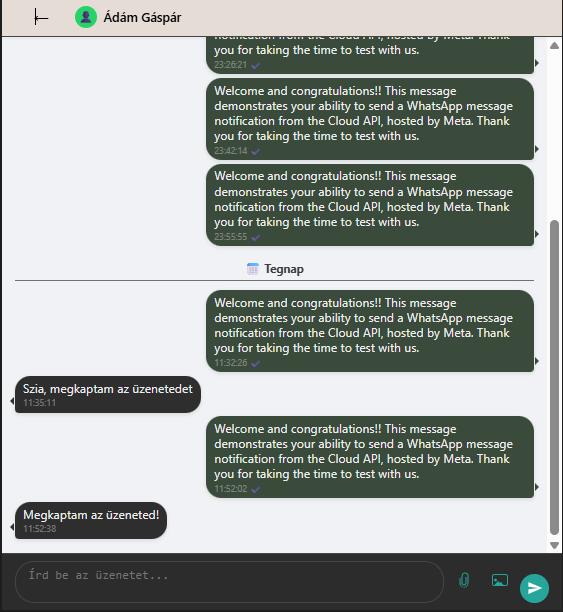
\includegraphics[width=0.95\textwidth]{images/conv-html.png}
\caption{A conv.html kontaktalapú beszélgetésnézete}
\label{fig:conv-html}
\end{figure}

A képernyőkép alapján látható, hogy a beszélgetésnézet célja a bejövő és kimenő üzenetek időrendi, olvasható visszaadása. A bejövő és kimenő üzenetek elkülönítése, az időrendi megjelenítés és a médiatartalmak értelmezhető kezelése mind azt szolgálja, hogy a felhasználó ne technikai naplót, hanem valódi beszélgetési előzményt lásson.

A beszélgetésnézetben ezt a frontendoldali értelmezést a \path{conv.html} üzenettípus szerinti feldolgozása valósítja meg. A következő egyszerűsített részlet azt mutatja, hogy a nézet külön kezeli a képeket, dokumentumokat, sablonos üzeneteket és szabad szöveges tartalmakat.

\begin{CodeBlock}
if (msg.type === 'image' || msg.type === 'media') {
  let src = normalizeMediaUrl(msg.media || msg.content || '');

  if (msg.type === 'media' && src && !isImageUrl(src)) {
    body =
    `<a href="${src}" target="_blank">Dokumentum megnyitása</a>`;
  } else {
    body = src
      ? `<img src="${src}" alt="Kép"
         style="max-width:100%; border-radius:6px;">`
      : '<em>Kép nem elérhető</em>';
  }

} else if (msg.type === 'document') {
  let link = normalizeMediaUrl(msg.media || msg.content || '');

  body = link
    ? `<a href="${link}" target="_blank">Dokumentum megnyitása</a>`
    : '<em>Dokumentum nem elérhető</em>';

} else if (msg.type === 'template') {
  const parsed = JSON.parse(msg.content || '{}');
  const tplName = parsed.template || 'ismeretlen_sablon';
  const paramValues = parsed.parameters || [];

  const templateData = templateMap[tplName];

  if (templateData && templateData.text) {
    let text = templateData.text;

    paramValues.forEach((val, i) => {
      const regex = new RegExp(`\\{\\{${i + 1}\\}\\}`, 'g');
      text = text.replace(regex, val);
    });

    body = `<div style="white-space:pre-wrap;">${text}</div>`;
  } else {
    body = '<div><em>Sablon nem található vagy üres.</em></div>';
  }

} else {
  const raw = msg.content?.trim() || '';
  body = questionMap[raw] || raw;
}
\end{CodeBlock}

A kódrészlet azért fontos, mert megmutatja, hogy a beszélgetésnézet nem nyers adatmezőket jelenít meg. A frontend először az üzenet típusát értelmezi, majd ehhez igazítja a megjelenítést. Kép esetén vizuális előnézet készül, dokumentum esetén megnyitható hivatkozás jelenik meg, sablonos üzenet esetén pedig a rendszer megpróbálja a sablon szövegét és a paramétereket emberileg olvasható üzenetté alakítani. Ez közvetlenül kapcsolódik ahhoz a fejlesztési célhoz, hogy a \path{conv.html} kommunikációs folyamatot mutasson meg.

\section{Kérdőív-szerkesztő és -küldő modul}

A WaccApp kérdőíves modulja a rendszer egyik legösszetettebb frontendrésze, mert itt a felületnek nemcsak egyszerű adatbevitelt kell biztosítania, hanem több lépésből álló kommunikációs folyamatokat kell szerkeszthetővé tennie A modul fejlesztése során két eltérő működési irány jelent meg. A \path{questionnaire.html} a szöveges vagy számalapú válaszlogikára épülő kérdőívek korábbi, rugalmasabb szerkesztési irányát képviseli, míg a \path{template.html}, a \path{template-menu.html} és a \path{template-single.html} a sablonos, gombos WhatsApp-kompatibilis kérdőívfolyamatok kezeléséhez kapcsolódik. A végleges bemutatásban a hangsúly a sablonos kérdőívlánc-szerkesztésre kerül, mert ez illeszkedik közvetlenebbül a WhatsApp Business Platform kötöttebb kommunikációs modelljéhez.

A \path{questionnaire.html} fejlesztési irányának szerepe abban állt, hogy megmutatta: a kérdőív nem kezelhető egyszerű kérdéslistaként. A szöveges vagy számalapú válaszokra épülő működésnél a kérdésekhez válaszlehetőségek és válaszfüggő következő lépések kapcsolódnak. Ez a felismerés később a sablonos kérdőívlánc-szerkesztésben is hasznosult, mert ott is ugyanaz az alapelv érvényesül: egy válasz csak akkor értelmezhető teljesen, ha ismert, hogy milyen következő kommunikációs lépést indít el.

Ebből következett, hogy a szöveges vagy számalapú kérdőíveknél a kérdéseket és válaszokat egymáshoz kapcsolódó szerkezeti elemekként kellett kezelni. Egy válasz csak akkor értelmezhető teljesen, ha ismert, hogy utána milyen következő kérdés következik, vagy a folyamat lezárul-e. Ha ez a kapcsolat hiányzik, akkor a kérdőív futás közben megszakadhat. Ezért a \path{questionnaire.html} nem csupán kitöltendő mezőket tartalmaz, hanem olyan szerkesztési helyzetet teremt, ahol a felhasználó a kérdéslánc logikáját is ellenőrizni tudja. Ez a saját frontendmegoldás azért lényeges, mert a kérdőív itt nem statikus tartalomként, hanem dinamikus kommunikációs útvonalként jelenik meg. A válaszfüggő kérdőívlogika egyszerűsített adatszerkezeti példája a 15.4. mellékletben látható, amely a kérdőíves gondolkodás alapját szemlélteti.

A sablonos kérdőívek működése ettől eltérő. A \path{template.html} a gombos, sablonalapú kérdőívfolyamatok szerkesztését támogatja, ahol a felhasználói válasz nem szabad szöveges bevitelként, hanem előre meghatározott gombos opcióként jelenik meg. A \path{template-menu.html} a sablonos feladatok közötti választást segíti, a \path{template-single.html} pedig az egyszerűbb sablonkészítési helyzetekhez kapcsolódik. Ez a különválasztás azért indokolt, mert az egyszerű sablonkészítés és a több lépésből álló sablonlánc szerkesztése nem ugyanaz a feladat. Az előbbi inkább egy adott üzenet struktúrájára koncentrál, az utóbbi viszont már egy teljes kérdőíves kommunikációs folyamatot kezel. 

A sablonos kérdőívfolyamatoknál a frontendnek alkalmazkodnia kell a WhatsApp Business Platform kötöttebb működéséhez is. A sablon neve, szövege, paraméterezése és a gombok logikája nem lehet teljesen szabad, mert a háttérben olyan platform működik, amely meghatározott formátumokat vár el. A \path{template.html} ezért olyan szerkesztési környezetet ad, amely egyszerre támogatja a felhasználói rugalmasságot és a platformlogika betartását. Ez a modul így nemcsak kényelmi szerkesztőfelület, hanem a hibás sablonláncok és megszakadó kérdőívfolyamatok megelőzésének eszköze is. [R1], [R2], [R3] 

A sablonos kérdőívfolyamatok esetében a \path{template.html} nézet mutatja meg, hogyan jelenik meg a gombos válaszokra és sablonláncokra épülő logika a frontendben. A képernyőkép azért fontos, mert a sablonos működés a WhatsApp Business Platform kötöttebb kommunikációs modelljéhez kapcsolódik.

\begin{figure}[H]
\centering
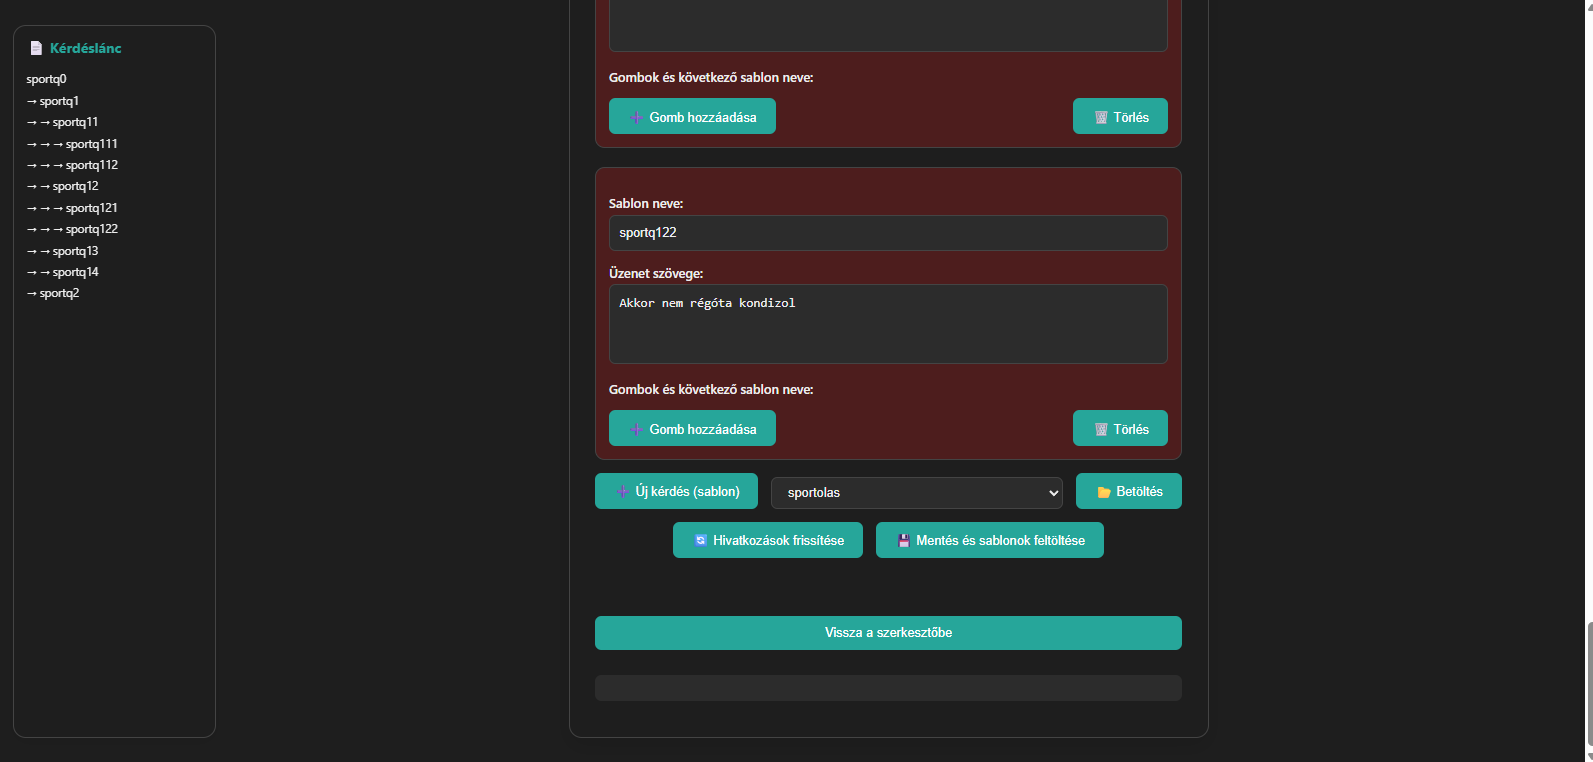
\includegraphics[width=0.95\textwidth]{images/template-html.png}
\caption{A template.html sablonos kérdőívlánc-szerkesztő felülete}
\label{fig:template-html}
\end{figure}

A \path{template.html} felületén a szerkesztés sablonokhoz, gombos válaszokhoz és következő lépésekhez kapcsolódó folyamat kialakítását jelenti. Ez a nézet jól mutatja, hogy a WaccApp frontendjében a sablonkezelés egy kommunikációs logika előkészítése. Emiatt a képernyőkép a kérdőíves modul saját fejlesztési súlyát is erősíti.

A kérdőíves modul értéke abban áll, hogy a WaccApp nemcsak elküldeni tud egy kérdést, hanem előtte lehetőséget ad a folyamat megtervezésére. A szöveges válaszlogika és a gombos sablonlogika párhuzamos kezelése azért erős saját fejlesztési elem, mert két különböző kommunikációs modellt tesz elérhetővé ugyanabban a rendszerben. A \path{questionnaire.html} rugalmasabb, szabadabb válaszokra épülő folyamatokat támogat, míg a \path{template.html} strukturáltabb, platformhoz igazított kérdőívlogikát valósít meg. A két nézet együtt adja a WaccApp kérdőíves működésének lényegét. 

\section{Szűrők és statisztikák}

A \path{filter.html} a WaccApp azon nézete, amely a korábban létrejött kommunikációs adatok visszakeresését és alapvető értelmezését támogatja. Ez a modul azért kap önálló szerepet, mert egy kommunikációs rendszerben az adatok értéke nem ér véget az üzenetek elküldésével vagy a válaszok beérkezésével. A felhasználónak később is szüksége lehet arra, hogy meghatározott címzett, időszak, üzenettípus vagy kérdőíves válasz alapján megtalálja a releváns eseményeket. A \path{filter.html} ezért nem egyszerű keresőoldal, hanem a WaccApp kommunikációs adatainak célzott értelmező felülete. 

A modul egyik legfontosabb sajátossága, hogy több szűrési feltételt képes együtt kezelni. A felhasználó név, telefonszám, üzenettípus, dátumintervallum, kérdőív, kérdés vagy válasz alapján is kereshet. Frontend szempontból ez azért összetett feladat, mert ezek a feltételek nem egymástól függetlenül hatnak. Egy dátumintervallum például szűkítheti az adott személyhez tartozó üzeneteket, az üzenettípus tovább pontosíthatja az eredményt, a kérdőívhez kapcsolódó mezők pedig a kommunikáció egy speciális részhalmazát emelhetik ki. A felületnek ezért úgy kell kezelnie a mezőket, hogy a felhasználó értelmezhető keresési helyzetet hozzon létre. 

Különösen fontos frontenddöntés volt a név és telefonszám összekapcsolása. A szűrőfelület fejlesztése közben hamar kiderült, hogy a két adat külön kezelése könnyen hibás keresési helyzetet teremthet. Ha a felhasználó egy ismert nevet választ ki, de mellette másik telefonszám marad a mezőben, akkor a rendszer technikailag ugyan lefuttathatja a keresést, az eredmény viszont félrevezető lehet. Emiatt a frontendben fontos döntés lett, hogy a név és a hozzá tartozó telefonszám egymást támogató mezőként működjön, ne pedig egymástól független szűrési adatként. Ez a részlet jól mutatja, hogy a \path{filter.html} nem csak mezőket sorol egymás alá, hanem a keresési logika helyességét is támogatja.

A név és telefonszám összekapcsolását a \path{filter.html} kliensoldali térképezéssel oldja meg. A beérkező és elküldött üzenetek feldolgozása közben a frontend név–telefonszám és telefonszám–név kapcsolatokat épít, majd ezek alapján szinkronizálja a szűrőmezőket.

\begin{CodeBlock}
contactMap = {};
nameToPhone = {};
phoneToName = {};

const incoming = inbox.map(m => {
  const phone = m.Phone_number;
  const name = m.Name || 'Ismeretlen';

  contactMap[phone] = name;
  nameToPhone[name] = phone;
  phoneToName[phone] = name;

  return {
    direction: 'received',
    name,
    phone,
    timestamp: new Date(m.Received_at),
    type: m.Type,
    content: m.Body
  };
});

nameSelect.addEventListener('change', () => {
  const name = nameSelect.value;
  const phone = nameToPhone[name] || '';
  phoneSelect.value = phone;
});

phoneSelect.addEventListener('change', () => {
  const phone = phoneSelect.value;
  const name = phoneToName[phone] || '';
  nameSelect.value = name;
});
\end{CodeBlock}

Ez a megoldás nem látványos, mégis fontos frontenddöntés. Ha a név és a telefonszám egymástól független mezőként működne, a felhasználó könnyen olyan keresést indíthatna, amelyben egy névhez hibás telefonszám társul. A szinkronizálás ezt a hibalehetőséget csökkenti, mert az egyik mező kiválasztása automatikusan igazítja a másikat. A \path{filter.html} így a keresési feltételek értelmezhetőségét is védi.

A dátumintervallum szerinti szűrés szintén lényeges része a modulnak. A felhasználó sok esetben nem egyetlen konkrét üzenetet keres, hanem egy adott időszak kommunikációs eseményeit szeretné áttekinteni. Ez különösen kérdőíves vagy kampányszerű használatnál fontos, ahol az eredmények időbeli alakulása is jelentéssel bírhat. A frontend feladata itt nemcsak két dátummező megjelenítése, hanem annak biztosítása is, hogy az intervallum értelmezhető legyen. Ha a kezdődátum későbbi, mint a záródátum, akkor a felületnek ezt hibás keresési helyzetként kell kezelnie, mert az ilyen lekérdezés félrevezető eredményt adhatna. 

Az eredmények megjelenítése a modul másik fontos része. A \path{filter.html} felületén a találatoknak olyan formában kell megjelenniük, hogy a felhasználó ne csak azt lássa, hogy léteznek adatok, hanem gyorsan értelmezni is tudja őket. A strukturált megjelenítés ebben a helyzetben azért indokolt, mert több metaadatot kell egyszerre figyelembe venni: a címzettet, az időpontot, az üzenettípust, a kérdőívet, a kérdést vagy a választ.

A \path{filter.html} képernyőképe a WaccApp visszakeresési és egyszerű válaszösszesítési működését mutatja be. A rendszer ezen része itt nem új kommunikációt indít, hanem a korábban keletkezett üzenetek és kérdőíves válaszok értelmezését támogatja.

\begin{figure}[H]
\centering
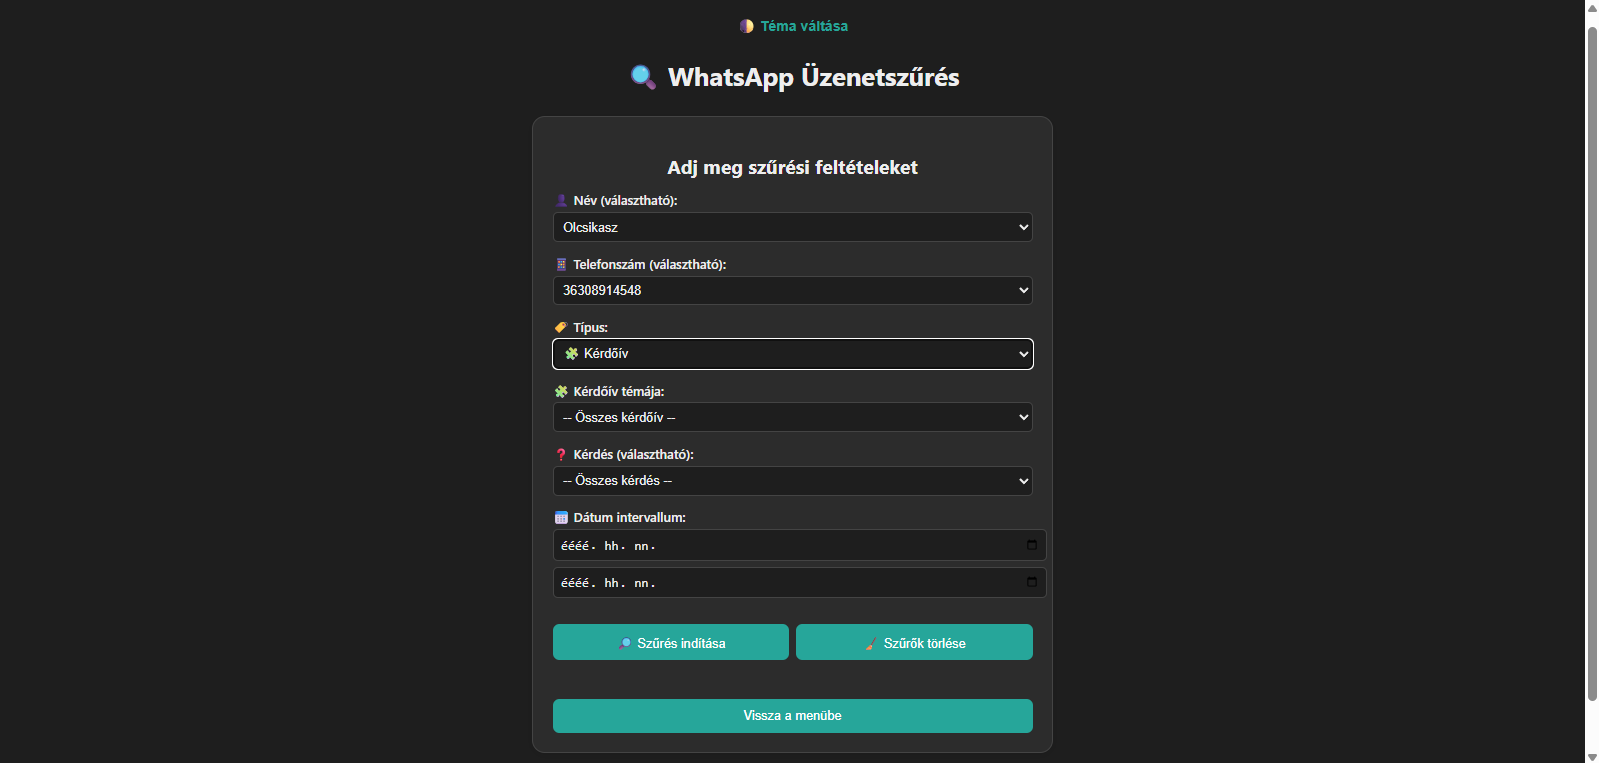
\includegraphics[width=0.95\textwidth]{images/filter-html.png}
\caption{A filter.html kérdőíves szűrési feltételeket kezelő nézete}
\label{fig:filter-html}
\end{figure}

A képernyőkép alapján látható, hogy a szűrőfelület többféle keresési szempontot kezel, például nevet, telefonszámot, dátumot, üzenettípust, kérdőívet vagy kérdést. A nézet célja, hogy a felhasználó a korábban létrejött kommunikációs és kérdőíves adatok között célzottan tudjon keresni. Az egyszerű válaszösszesítés ehhez a szűrési logikához kapcsolódik, vagyis a kérdőíves adatok értelmezését segítő kiegészítőként jelenik meg.

A modulban megjelenő alapvető statisztikai funkció nem teljes analitikai rendszert jelent, hanem kérdőíves válaszok egyszerű darabszám szerinti összesítését. Ennek működését a következő egyszerűsített kódrészlet szemlélteti.

\begin{CodeBlock}
function collectAnswerStats(theme, qid) {
  const flow = window.__flowCache?.[theme] || {};
  const node = flow[qid] || {};
  const options = Object.keys(node.next || {});

  const respondents = {};
  const otherKey = '__OTHER__';

  function addAnswer(key, phone) {
    if (!respondents[key]) respondents[key] = new Set();
    respondents[key].add(phone);
  }

  allMessages.forEach((msg, index) => {
    if (isQuestionMessage(msg, theme, qid)) {
      const reply = findFirstReplyAfter(index, allMessages);
      if (!reply) return;

      const answer = normAnswer(reply.content || '');
      const known = options.find(opt => normAnswer(opt) === answer);
      addAnswer(known || otherKey, reply.phone);
    }
  });

  const counts = {};
  options.forEach(opt => {
    counts[opt] = respondents[opt]?.size || 0;
  });

  if (respondents[otherKey]?.size) {
    counts[otherKey] = respondents[otherKey].size;
  }

  return { counts, respondents };
}
\end{CodeBlock}

A válaszösszesítés lényege, hogy a frontend a kérdőív adott kérdéséhez megkeresi a hozzá tartozó első választ, majd az ismert válaszlehetőségekhez vagy az „Egyéb” kategóriához sorolja. A Set használata azért hasznos, mert egy válaszopcióhoz címzettenként számolja a válaszadókat, nem egyszerűen nyers üzenetszámot jelenít meg.

Amikor a felhasználó kérdőíves szűrést alkalmaz, és kiválaszt egy konkrét kérdést, a felület képes megmutatni, hogy az adott válaszlehetőségekre hány válasz érkezett. A válaszok között megjelenhet az összes válasz darabszáma, az egyes ismert válaszopciókhoz tartozó darabszám, valamint egy „Egyéb” kategória is azokhoz az értékekhez, amelyek nem illeszkednek az előre ismert válaszlehetőségekhez.

Ez a megoldás elsősorban kérdőíves válaszok gyors áttekintésére alkalmas. A célja az, hogy a felhasználó rögtön lássa, mely válaszok fordultak elő, és azokhoz körülbelül mekkora válaszadói kör tartozik. A felület a kiválasztott válaszhoz kapcsolódó személyeket vagy telefonszámokat is meg tudja jeleníteni, így az összesítés nem szakad el a konkrét kommunikációs adatoktól. Ez különösen hasznos akkor, ha a felhasználó nemcsak az arányokra kíváncsi, hanem arra is, hogy egy adott válasz mely címzettekhez kapcsolódott.

Fontos korlát ugyanakkor, hogy a WaccApp jelenlegi formájában nem tartalmaz diagramokat, idősoros kimutatásokat, exportálható riportokat vagy részletes kampányelemzést. Az üzenettípus, dátumintervallum, név, telefonszám, kérdőív és válasz szerinti szűrés támogatja az adatok célzott visszakeresését, de ezek nem alkotnak teljes értékű statisztikai dashboardot. A modul ezért inkább egyszerű frontendoldali értelmező és visszakereső felületként értékelhető, amely a későbbi fejlettebb statisztikai funkciók alapját adhatja.

A szűrési és válaszösszesítési modul tehát összeköti a WaccApp operatív és értelmező oldalát. Az \path{index.html} és a kérdőíves oldalak létrehozzák vagy elindítják a kommunikációs eseményeket, a \path{messages.html}, a \path{sent-messages.html} és a \path{conv.html} visszakövethetővé teszik azokat, a \path{filter.html} pedig célzott kereséssel és egyszerű válaszösszesítéssel segíti az utólagos feldolgozást. Ez a modul azért fontos, mert általa a WaccApp nemcsak küldőfelületként működik, hanem a kommunikációs és kérdőíves adatok későbbi alapvető értelmezését is támogatja.


\section{Média- és fájlkezelés}

A média- és fájlkezelés a WaccApp kommunikációs működésének kiterjesztése. A rendszer nem kizárólag szöveges tartalmak továbbítására készült, hanem képek és dokumentumok kezelésére is alkalmas. Ez a funkció elsősorban az \path{index.html} küldőfelülethez, a \path{conv.html} beszélgetésnézethez, valamint a public/uploads és a public/sent\_media mappákhoz kapcsolódik. A modul jelentősége abban áll, hogy a fájlok nem különálló technikai mellékletekként jelennek meg, hanem a kommunikációs folyamat részeként. 

Az \path{index.html} oldalhoz kapcsolódó fájlkezelés a kiválasztással indul. A felhasználó megadja a címzettet, kiválasztja a továbbítandó fájlt, majd a rendszer a küldési folyamat részeként kezeli azt. Frontend szempontból itt az egyik legfontosabb döntés az, hogy a fájlkiválasztás ne vak művelet legyen. A felhasználónak még a küldés előtt érzékelnie kell, hogy milyen állományt választott ki, és az alkalmas-e a továbbításra. Képek esetében ezt vizuális előnézet segítheti, dokumentumok esetében pedig a fájlnév és a típus megjelenítése adhat ellenőrzési lehetőséget. 

A public/uploads és a public/sent\_media mappák eltérő szerepet töltenek be a rendszer működésében. Az uploads a feltöltött vagy előkészített állományokhoz kapcsolódik, míg a sent\_media az elküldött médiaelemek visszakövetésében kap szerepet. Ez a különbség frontend szempontból azért fontos, mert a fájlkezelés nem zárul le a kiválasztás és elküldés pillanatában. A felhasználó számára az is lényeges, hogy később a beszélgetésben vagy az előzmények között értelmezhetően vissza tudja nézni, milyen médiatartalom került továbbításra. 

A \path{conv.html} oldal különösen fontos szerepet kap a médiafájlok megjelenítésében. Ha egy elküldött kép csak hivatkozásként jelenne meg, a felhasználónak külön meg kellene nyitnia, hogy megértse, milyen tartalomról van szó. A vizuális megjelenítés ezzel szemben azonnal értelmezhetővé teszi a médiát a beszélgetés kontextusában. Ez nem apró esztétikai részlet, hanem konkrét használhatósági különbség. Egy beszélgetés visszakövetésekor a felhasználó nem fájlelérési útvonalakat akar olvasni, hanem azt szeretné látni, milyen tartalom ment ki vagy érkezett be az adott kommunikációs folyamatban. 

A média- és fájlkezelésnél a hibamegelőzés is konkrét formában jelenik meg. A nem támogatott fájltípus, a hibás kiválasztás vagy a hiányzó állomány olyan helyzet, amelyet célszerű már a küldési folyamat elején kezelni. A frontend feladata itt az, hogy a felhasználó ne csak a szerveroldali elutasítás után találkozzon a problémával, hanem már a kiválasztás vagy küldés előkészítése során visszajelzést kapjon. Ez csökkenti a félreküldés, a sikertelen feltöltés és a bizonytalan felhasználói helyzetek esélyét. [R13], [R14] 

A modul korlátja, hogy a fájlkezelés frontendoldalon csak részben ellenőrizhető. A tényleges továbbítás, tárolás és WhatsApp-platformszintű feldolgozás a háttérrendszerhez és a külső szolgáltatáshoz kapcsolódik. A frontend mégis jelentős szerepet vállal abban, hogy a felhasználó a küldés előtt és után is értelmezhető információt kapjon. A médiafunkció ezért nem egyszerű csatolmánykezelésként, hanem a kommunikáció vizuális gazdagításaként jelenik meg a WaccApp-ban. 

\section{Időzített kampányok és ütemezett küldések}

Az időzített küldések modulja az \path{index.html} küldési folyamatának kiterjesztéseként értelmezhető. A rendszer ezen a ponton nem új, teljesen különálló kommunikációs felületet hoz létre, hanem az azonnali küldés logikáját egészíti ki azzal a lehetőséggel, hogy a felhasználó egy későbbi időponthoz kösse a művelet végrehajtását. Ez a funkció szöveges üzenet, sablon, kérdőív vagy médiafájl esetében is értelmezhető, de frontend szempontból minden esetben ugyanaz a központi kérdés: a felhasználó ne csak tartalmat adjon meg, hanem a végrehajtás időpontját is egyértelműen meghatározza. 

Az időzítés felületi szempontból azért összetett, mert az időpont önmagában nem elegendő adat. Egy időzített szöveges üzenethez szükséges a címzett és az üzenettartalom, egy időzített sablonküldéshez a sablon és a paraméterek, egy kérdőívindításhoz a kiválasztott kérdőív, médiafájl esetén pedig a továbbítandó állomány. A frontendnek ezért az időzítést nem önálló mezőként, hanem a választott küldési típushoz kapcsolódó kiegészítő adatként kell kezelnie. Ez a megoldás biztosítja, hogy az időzítés ne váljon elszakított beállítássá, hanem a konkrét kommunikációs művelet részeként működjön. 

A modul egyik legfontosabb frontendfeladata az időpont értelmezhetőségének ellenőrzése. Ha a felhasználó nem ad meg időpontot, múltbeli időpontot választ, vagy olyan adatot rögzít, amely nem kapcsolható értelmesen a kiválasztott küldési módhoz, akkor a rendszernek ezt még a mentés előtt jeleznie kell. Ez különösen fontos, mert időzített műveleteknél a hiba sokszor nem azonnal derülne ki. Egy rosszul beállított időpont vagy hiányos tartalom később okozna sikertelen küldést, amikor a felhasználó már nem feltétlenül figyeli aktívan a folyamatot. 

Az időzített küldések sajátossága, hogy a művelet indítása és tényleges végrehajtása időben elválik egymástól. Az azonnali üzenetküldésnél a felhasználó rövid időn belül visszajelzést vár a küldés sikeréről vagy hibájáról. Időzítésnél viszont először a rögzítés sikeressége, később pedig a tényleges végrehajtás állapota válik fontossá. Emiatt a frontendnek nemcsak a mentés pillanatában kell visszajelzést adnia, hanem a későbbi státuszok értelmezhetőségét is támogatnia kell. A várakozó, elküldött vagy sikertelen állapotok a felhasználó számára azt mutatják meg, hogy a korábban beállított kommunikációs művelet hol tart az életciklusában. 

A modul elnevezésében szereplő kampánylogika ezért nem teljes értékű marketingautomatizálási rendszert jelent, hanem a WaccApp kommunikációs folyamatainak időbeli tervezhetőségét. Ez fontos különbség, mert a frontend jelenlegi szerepe nem egy komplex kampánymenedzsment-dashboard kiváltása, hanem az, hogy az azonnali küldések mellett előre ütemezhető műveleteket is kezelhetővé tegyen. A megoldás gyakorlati értéke abban áll, hogy a felhasználó nemcsak reagálni tud egy kommunikációs helyzetre, hanem előre is beállíthat bizonyos küldési folyamatokat. 

Az időzített küldések modulja tehát a WaccApp frontendjében a kommunikációs kontroll kiterjesztéseként jelenik meg. Az \path{index.html} továbbra is a központi indítófelület marad, de a küldés ideje már nem feltétlenül azonos a művelet rögzítésének idejével. Ez a különbség indokolja az időpontmező, a hozzá kapcsolódó validáció, valamint a későbbi státuszkövetés szerepét. 

\section{A modulok együttműködése a WaccApp frontendjében}

A WaccApp kiemelt moduljai nem önálló, egymástól független funkciók, hanem egy közös kommunikációs folyamat különböző szakaszait támogatják. A \path{login.html} és a \path{menu.html} a rendszer használatának keretét adják: előbbi a belépési pontot, utóbbi a főbb nézetek közötti eligazodást biztosítja. Az \path{index.html} elindítja az üzenetküldést, a kérdőívindítást, a médiaküldést vagy az időzített műveletet. A \path{messages.html} és a \path{sent-messages.html} listaalapú áttekintést ad a kommunikációs eseményekről. A \path{conv.html} egy adott kontakt beszélgetését rendezi értelmezhető folyamatba. A \path{questionnaire.html} és a sablonkezelő oldalak a kérdőíves kommunikáció előkészítését szolgálják, a \path{filter.html} pedig az utólagos visszakeresést és alapvető elemzést támogatja. 

Ez az együttműködés teszi a WaccApp frontendjét többé egyszerű oldalak gyűjteményénél. A rendszerben egy művelet gyakran több nézeten keresztül válik teljessé. Egy kérdőív például először a szerkesztőfelületen jön létre, később az \path{index.html} oldalról indítható, a válaszok a kommunikációs előzményekben jelennek meg, végül a \path{filter.html} segítségével visszakereshetők. Hasonló logika figyelhető meg a médiaküldésnél is: a fájl kiválasztása és küldése az indítófelülethez kapcsolódik, de az elküldött tartalom valódi értelme a beszélgetésnézetben válik láthatóvá. 

A fejezet szerepe ezért az, hogy megmutassa a WaccApp saját frontendmegoldásait működés közben. A korábbi fejezetekben szereplő követelmények, UX-döntések és architekturális alapok itt konkrét modulokká állnak össze. Az üzenetküldés, a kérdőívkezelés, a szűrés, a médiafájl-kezelés és az időzítés külön-külön is értelmezhető funkciók, de a rendszer gyakorlati értékét az adja, hogy ezek egymáshoz kapcsolódva támogatják a WhatsApp-alapú kommunikáció teljesebb kezelését. Ez a moduláris együttműködés alapot biztosít a következő fejezethez, amely már azt mutatja be, hogy a frontend nézetei milyen API-kapcsolatokon keresztül működnek együtt a háttérrendszerrel. [R1], [R10], [R13], [R14] 
